\documentclass[8pt, a4paper, landscape, includeheadfoot]{extarticle}

% Verwendete Pakete

	\usepackage[utf8]{inputenc}
	\usepackage[top=0.2cm, 
	            bottom=0.01cm, 
	            left=0.5 cm, 
	            right=0.5 cm, 
	            footskip = 2.9pt]{geometry}
	\usepackage{babel} % set language to new german
	\usepackage{amsmath}
	\usepackage{amsfonts}
	\usepackage{lmodern}
	\usepackage{graphicx}
	\setlength{\parindent}{0pt}
	\usepackage{ulem} %option rausgenommen
	\usepackage[dvipsnames]{xcolor}%option "table" raus
	\usepackage{enumitem}
	\usepackage{mathabx}
	\usepackage{enumitem}
	\usepackage{colortbl}
	\usepackage{mathtools}
	\usepackage{wallpaper}
	\usepackage{changepage}
	\usepackage{tikz}
	\usepackage{tabularx}
	\usepackage[skins]{tcolorbox}
	\usepackage{lipsum}
	\usepackage{multicol}
	\usepackage{multirow}
	\usepackage{letltxmacro}
	\usepackage{tabularx}
	\usepackage{float}
    \usepackage{amssymb, physics}
    \usepackage{empheq}
    \usepackage{textcomp} % gensymb dependency
    \usepackage{calc} % Multiplikation mit werten ermöglichen
    \usepackage[makeroom]{cancel} %Terme durchstreichen
    \usepackage{mathtools}
    \usepackage{sidecap} %für Bild und Text nebeneinander
    %\usepackage{gensymb} % Degree celcius symbol
    \usepackage{fancyhdr} % Kopfzeile
    \usepackage{romannum} % roman numbers
	\usepackage{makecell} % zeilenumbruch in tabellen


% Spalteneinstellungen

\setlength\columnsep{5mm}
\setlength{\columnseprule}{0.5pt}

%FBOX Einstellungen

\setlength{\fboxrule}{0.5pt}

%Kopf und Fusszeile 

\setlength{\headsep}{0.5em}
\setlength{\footskip}{2.9pt}

\pagestyle{fancy}
\fancyhf{}
\lhead{\textbf{\Subject}}
\chead{Page \thepage{}}
\rhead{\CustomAuthor}
\cfoot{}

% Farbe

\def \customColor {PineGreen}

% Bullet-Symbol für Aufzählungen
\renewcommand\textbullet{\ensuremath{\bullet}}

% Eingekreiste Nummern für Aufzählungen
\newcommand*\circled[1]{\tikz[baseline=(char.base)]{
        \node[shape=circle,draw,inner sep=1.2pt] (char) {#1};}}

% Schriftart
\renewcommand{\familydefault}{\sfdefault}

%Tabelle Horiz. Grösse
\renewcommand{\arraystretch}{1.5}

%Einheiten
\newcommand{\Einheit}[1]{
$\bigl[ #1 \bigr]$
}

\newcommand{\EinheitBruch}[2]{
$\bigl[ \frac{#1}{#2} \bigr]$
}

\newcommand{\Umbruch}{\vfill\null\columnbreak}

% Titel-Block	
\newcommand{\Header}[3]{
	\begin{tcolorbox}  [arc = 0mm, 
	                    colback = \customColor!50!black, 
	                    colframe = \customColor!50!black, 
	                    valign = center, 
	                    fontupper=\color{white}]
		\large \center \textbf{#1} \par
		\huge \textbf{#2} \par 
		\vskip 5pt 
		\large #3 \par
		\vskip 3pt 
		\small Version: \today
	\end{tcolorbox}
	}

%Teil-Block
\newcommand{\Abschnitt}[1]{
	\begin{tcolorbox} [arc = 0mm,
						colback = \customColor!50!black,
						colframe = \customColor,
						valign = center,
						before skip = 3mm,
						leftright skip = -0.5mm,
						after skip = 1 mm,
						bottomrule = 0 mm,
						toprule = 0 mm,
						leftrule = 0 mm,
						rightrule = 0 mm,
						fontupper=\color{white}
						]
		\centering\Large\textbf{#1}
	\end{tcolorbox}
}

% Überschrift
\renewcommand{\section}[1]{
	\begin{tcolorbox}[
			arc=0mm,
			colback=\customColor!50!black,
			colframe=white,
			bottomrule = 0 mm,
			toprule = 0 mm,
			leftrule = 0 mm,
			rightrule = 0 mm,
			valign=center,
			left=0.5mm,
			top= 0.7 mm,
			bottom= 0.7 mm,
			fontupper=\color{white},
			before skip = 1mm,
			leftright skip = -0.5mm,
			after skip = 1 mm]

		\textbf{#1}
	\end{tcolorbox}
	}

% Abschnitt	
\renewcommand{\subsection}[1]{
\begin{tcolorbox}[
            		arc=0mm,
            		colback=\customColor!50,
            		colframe=white,
            		bottomrule = 0 mm,
            		toprule = 0 mm,
            		leftrule = 0 mm,
            		rightrule = 0 mm,
            		valign=center,
            		left=0.5mm,
            		top=0.2mm,
            		bottom=0.2mm,
            		before skip = 1mm,
            		leftright skip = -0.5mm,
            		after skip = 1mm]
	\small \textbf{#1}
\end{tcolorbox}
}

\renewcommand{\subsubsection}[2]{
\begin{tcolorbox}[
            		arc=0mm,
            		colback=gray!50,
            		colframe=white,
            		bottomrule = 0 mm,
            		toprule = 0 mm,
            		leftrule = 0 mm,
            		rightrule = 0 mm,
            		valign=center,
            		left=0.5mm,
            		top=0.2mm,
            		bottom=0.2mm,
            		before skip = 1mm,
            		leftright skip = -0.5mm,
            		after skip = 1mm]
	\small #1 \hfill #2
\end{tcolorbox}
}

%MATH-BOX, optional commands in {}
\newtcbox{\mathbox}[1][]{%
    nobeforeafter, 
    tcbox raise base, 
    colframe=blue!30!black,
    colback=blue!20, 
    boxrule=1pt,
    arc=1mm,
    before skip = 0mm,
    right = 1mm,
    left=1mm,
	top=0.5mm,
	bottom=0.5mm,
    #1}
    
\newtcbox{\mathboxnoback}[1][]{%
    nobeforeafter, 
    tcbox raise base, 
    colframe=black,
    colback=white,
    boxrule=1pt,
    arc=1mm,
    before skip = 0mm,
    right = 1mm,
    left=1mm,
	top=0.5mm,
	bottom=0.5mm,
    #1}
    
\newcommand{\textbox}[1]{
\tcbox[
		arc=1mm,
		colback=blue!20,
		colframe=blue!30!black,
		arc=1mm,
		boxrule=1pt,
		right = 1mm,
        left=1mm,
	    top=0.5mm,
	    bottom=0.5mm,
		before skip = 1mm,
		after skip = 2 mm
		]
{    
	#1
}
}

\newcommand{\textboxmithead}[2]{
\begin{tcolorbox}[
		arc=1mm,
		colback=blue!20,
		colframe=blue!30!black,
		arc=1mm,
		boxrule=1pt,
		left=1mm,
		top= 1 mm,
		bottom= 1 mm,
		before skip = 2mm,
		leftright skip = 8mm,
		after skip = 2 mm
		]
    \centering{\textbf{#1}\par}
	#2
\end{tcolorbox}
}

\newtcolorbox{titlebox}[1][]{
        fonttitle=\bfseries, 
        colbacktitle=gray!80,
        enhanced,
        attach boxed title to top center={yshift=-2mm},
        colframe=black,
        colback=white,
        boxrule=1pt,
        arc=1mm,
        before skip = 2mm,
        right = 1mm,
        left=1mm,
    	top=0.5mm,
    	bottom=0.5mm,
        title=#1}



\def \Subject {CS229 - Machine Learning}
\def \CustomTitle {Linear Algebra \& Probability}
\def \CustomAuthor {Tim Reinhart - rtim@stanford.edu}

\begin{document}
\pagenumbering{arabic}
\begin{multicols*}{4}
	\Header{\Subject}{\CustomTitle}{\CustomAuthor}

	\section{Matrices}

	\subsection{Matrix Multiplication}

	Matrices can be multiplied with each other in the following manner:

	\begin{center}
		\fbox{
			$A \cdot B = C \hspace{5pt} \Rightarrow \hspace{5pt} c_{ik} = \sum_{j=1}^n a_{ij} \cdot b_{jk}$
		}
	\end{center}

	\begin{center}
		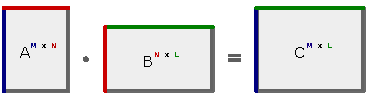
\includegraphics[width = 0.95 \columnwidth]{0_images/Matrixmultiplikation.pdf}
	\end{center}

	\textbf{Associative \& Distributive Laws:}

	\begin{center}
		\parskip3pt
		\begin{align}
			(A\cdot B) \cdot C & = A \cdot (B \cdot C) \nonumber   \\
			(A + B) \cdot C    & = A \cdot C + B \cdot C \nonumber \\
			A \cdot (C + D)    & = A \cdot C + A \cdot D \nonumber
		\end{align}
	\end{center}
	\textbf{Warning!} The commutative law does not apply! Generally, $A\cdot B \neq B \cdot A$.

	\subsection{Transpose}

	The transpose of a matrix is obtained by "mirroring" it along its diagonal.

	\begin{center}
		\textbf{Example:}
		$\begin{pmatrix}
				a & b \\
				c & d \\
				e & f \\
			\end{pmatrix}^T
			=
			\begin{pmatrix}
				a & c & e \\
				b & d & f \\
			\end{pmatrix}$
	\end{center}

	\textbf{Calculation Rules:}

	\vspace{-5mm}
	\begin{minipage}[t]{0.49 \columnwidth}
		\begin{align}
			(A + B)^T     & = A^T + B^T \nonumber     \\
			(A \cdot B)^T & = B^T \cdot A^T \nonumber \\
			(c \cdot A)^T & = c \cdot A^T \nonumber   \\
			(A^T)^T       & = A \nonumber
		\end{align}
	\end{minipage}
	\begin{minipage}[t]{0.49 \columnwidth}
		\begin{align}
			(A^T)^{-1} & = (A^{-1})^T \nonumber \\
			rank(A^T)  & = rank(A) \nonumber    \\
			det(A^T)   & = det(A) \nonumber     \\
			eig(A^T)   & = eig(A) \nonumber
		\end{align}
	\end{minipage}


	\subsection{Inverse}

	The inverse \( A^{-1} \) of \( A \) reverses a multiplication with \( A \). When you multiply \( A \) with \( A^{-1} \), you get the identity matrix.

	\textbf{Properties:}

	\begin{itemize}[leftmargin=0.29cm, itemsep=0pt]
		\item Only square matrices can be invertible.
		\item An invertible matrix is called \textbf{regular}, a non-invertible one \textbf{singular}.
		\item The inverse is unique.
		\item \( A \) is invertible if and only if \( A \) has full rank.
		\item \( A \) is invertible if and only if \( A^T \) is invertible.
		\item \( A \) is symmetric if and only if \( A^{-1} \) is symmetric.
		\item \( A \) is a triangular matrix if and only if \( A^{-1} \) is a triangular matrix.
		\item \( A \) is invertible if and only if \( \text{det}(A) \neq 0 \).
		\item \( A \) is invertible if and only if no eigenvalue \( \lambda = 0 \).
		\item \( A \) and \( B \) are invertible implies \( AB \) is invertible.
	\end{itemize}

	\textbf{Calculation rules:}

	\vspace{-5mm}
	\begin{minipage}[t]{0.49 \columnwidth}
		\begin{align}
			I^{-1}          & = I\nonumber                    \\
			(A^{-1})^{-1}   & = A \nonumber                   \\
			(A^k)^{-1}      & = (A^{-1})^k \nonumber          \\
			(c\cdot A)^{-1} & = c^{-1} \cdot A^{-1} \nonumber \\
			(A\cdot B)^{-1} & = B^{-1} \cdot A^{-1} \nonumber
		\end{align}
	\end{minipage}
	\begin{minipage}[t]{0.49 \columnwidth}
		\begin{align}
			(A^T)^{-1}   & = (A^{-1})^T \nonumber  \\
			rang(A^{-1}) & = rang(A) \nonumber     \\
			det(A^{-1})  & = det(A)^{-1} \nonumber \\
			eig(A^{-1}   & = eig(A)^{-1} \nonumber
		\end{align}
	\end{minipage}

	\subsection{Matrix Tricks}

	\textbf{Probability Rules for Matrices:}

	• Pull Matrix Multiply out of Variance:
	$$
		Var[Mx] = MVar[x]M^T
	$$

	\subsection{Eigenvalues and Eigenvectors}

	\begin{empheq}[box = \mathboxnoback]{align*}
		\text{Eigenvalues of A: } \det(A - \lambda\cdot I) = 0
	\end{empheq}

	\textbf{Verify Computation}

	\begin{itemize}[leftmargin=0.29cm, itemsep=0.5pt]
		\item Trace(A) = \( a_{11} + a_{22} + \dots + a_{nn} = \sum \lambda_i \)
		\item det(A) = product of \( \lambda_i \)
	\end{itemize}

	\textbf{Eigenvectors: } Kernel of the matrix $A - \lambda_i\cdot I$, where \( \lambda_i \) is the eigenvalue corresponding to the eigenvector.

	\subsection{Determinant}

	\textbf{Block Sentence for Determinant Computation}

	\begin{center}
		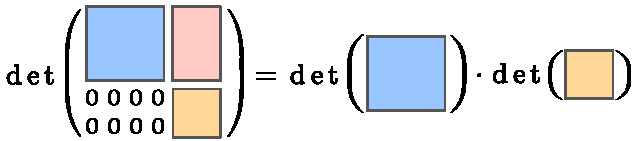
\includegraphics[width = 0.8 \columnwidth]{0_images/Blocksatz.pdf}
	\end{center}

	\section{Positive (Semi-)Definite Matrices}
	\subsection{Definitions}
	A symmetric matrix \( A \in \mathbb{R}^{n \times n} \) is called:
	\begin{itemize}
		\item \textbf{Positive Semi-Definite (PSD)} if for any non-zero vector \( \mathbf{x} \in \mathbb{R}^n \), we have \( \mathbf{x}^T A \mathbf{x} \geq 0 \).
		\item \textbf{Positive Definite (PD)} if for any non-zero vector \( \mathbf{x} \in \mathbb{R}^n \), \( \mathbf{x}^T A \mathbf{x} > 0 \).
	\end{itemize}

	\subsection{Properties}
	\begin{itemize}
		\item All eigenvalues of a PSD matrix are non-negative, and those of a PD matrix are positive.
		\item A matrix is PSD if and only if it can be written as \( B^T B \), where \( B \) is any matrix.
		\item If \( A \) is PD (or PSD), then so is \( A^{-1} \) (if \( A \) is invertible).
		\item For any matrix \( A \), the matrices \( A^T A \) and \( AA^T \) are PSD.
		\item The sum of two PSD matrices is also PSD.
	\end{itemize}

	\subsection{Checking for Positive (Semi-) Definiteness}
	Determining if a matrix is PSD or PD can be done in several ways:

	\begin{itemize}
		\item \textbf{Eigenvalue Criterion:} A symmetric matrix is PSD if and only if all its eigenvalues are non-negative. It is PD if all eigenvalues are positive.
		\item \textbf{Principal Minors:} A symmetric matrix \( A \) is PD if all its leading principal minors (determinants of the top-left \( k \times k \) submatrix, \( 1 \leq k \leq n \)) are positive. For PSD, all leading principal minors should be non-negative.
		\item \textbf{Cholesky Decomposition:} A matrix is PD if and only if it has a Cholesky decomposition. For numerical algorithms, attempting a Cholesky decomposition and checking for failure can be an effective way to test for positive definiteness.
	\end{itemize}

	\section{Matrix Calculus}
	\subsection{Gradient}
	The gradient of a scalar function $f: \mathbb{R}^n \rightarrow \mathbb{R}$ with respect to a vector $\mathbf{x} \in \mathbb{R}^n$ is a vector of partial derivatives:
	$$
		\nabla f(\mathbf{x}) = \begin{pmatrix}
			\frac{\partial f}{\partial x_1} \\
			\frac{\partial f}{\partial x_2} \\
			\vdots                          \\
			\frac{\partial f}{\partial x_n}
		\end{pmatrix}
	$$

	\subsection{Hessian}
	The Hessian matrix of a scalar-valued function $f: \mathbb{R}^n \rightarrow \mathbb{R}$ is a square matrix of second-order partial derivatives:
	$$
		H(f)(\mathbf{x}) = \begin{pmatrix}
			\frac{\partial^2 f}{\partial x_1^2}            & \frac{\partial^2 f}{\partial x_1 \partial x_2} & \cdots & \frac{\partial^2 f}{\partial x_1 \partial x_n} \\
			\frac{\partial^2 f}{\partial x_2 \partial x_1} & \frac{\partial^2 f}{\partial x_2^2}            & \cdots & \frac{\partial^2 f}{\partial x_2 \partial x_n} \\
			\vdots                                         & \vdots                                         & \ddots & \vdots                                         \\
			\frac{\partial^2 f}{\partial x_n \partial x_1} & \frac{\partial^2 f}{\partial x_n \partial x_2} & \cdots & \frac{\partial^2 f}{\partial x_n^2}
		\end{pmatrix}
	$$

	\subsection{Examples}

	\subsubsection{\( f(\mathbf{x}) = \mathbf{A}\mathbf{x} \)\hfill $\mathbf{A}\in\mathbb{R}^{m\times n}$}{}

	Gradient:
	$$
		\nabla f = \mathbf{A}^T
	$$

	\subsubsection{\( f(\mathbf{x}) = \mathbf{x}^T\mathbf{A}\mathbf{x} \)\hfill $\mathbf{A}\in\mathbb{R}^{m\times n}$}{}

	Gradient:
	$$
		\nabla f = (\mathbf{A} + \mathbf{A}^T)\mathbf{x}
	$$

	Hessian:
	$$
		H(f) = \mathbf{A} + \mathbf{A}^T
	$$

	\subsubsection{Linear Regression Loss (\( \ell_2 \) \textbf{norm})}{}
	For the loss function \( L(\mathbf{w}) = ||\mathbf{y} - \mathbf{X}\mathbf{w}||^2 \):

	Gradient:
	$$
		\nabla L = -2\mathbf{X}^T(\mathbf{y} - \mathbf{X}\mathbf{w})
	$$

	Hessian:
	$$
		H(L) = 2\mathbf{X}^T\mathbf{X}
	$$


	\subsubsection{Logistic Regression Loss}{}

	\begin{itemize}
		\item Binary classification with labels \( y_i \in \{0, 1\} \)
		\item Predicted probabilities \( p_i = \frac{1}{1 + e^{-\mathbf{x}_i^T \mathbf{w}}} \)
		\item \( L(\mathbf{w}) = -\sum_{i}[y_i \log(p_i) + (1-y_i) \log(1 - p_i)] \)
	\end{itemize}

	Gradient:
	$$
		\nabla L = \mathbf{X}^T(\mathbf{p} - \mathbf{y})
	$$

	Hessian:
	$$
		H(L) = \mathbf{X}^T \mathbf{S} \mathbf{X}
	$$

	where \( \mathbf{S} \) is a diagonal matrix with \( S_{ii} = p_i (1 - p_i) \).


	\section{Basic Probability}
	\subsection{Bayes Theorem}

	$$
		P(X{=}x | Y{=}y) = \frac{P(Y{=}y | X{=}x) P(X{=}x)}{P(Y{=}y)}
	$$

	Where:
	\begin{itemize}
		\item $P(X{=}x | Y{=}y)$ is the posterior probability: the probability of event $X{=}x$ given that $Y{=}y$ has occurred.
		\item $P(Y{=}y | X{=}x)$ is the likelihood: the probability of observing $Y{=}y$ given $X{=}x$.
		\item $P(X{=}x)$ is the prior probability: the initial belief about $X{=}x$.
		\item $P(Y{=}y)$ is the marginal probability: the total probability of observing $Y{=}y$ under all possible outcomes of $X$.
	\end{itemize}
	\subsubsection{Law of Total Probability}

	A key concept related to Bayes' Theorem is the Law of Total Probability. It is useful for calculating $P(Y{=}y)$, the marginal probability in Bayes' formula, especially when dealing with compound events. The law states:

	$$
		P(Y{=}y) = \sum_{i} P(Y{=}y | X{=}x_i) P(X{=}x_i)
	$$

	Where $X{=}x_i$ represents all disjoint outcomes that cover the sample space. In the context of Bayes' Theorem, it's used to marginalize over the different possible states of knowledge or evidence.

	\subsubsection{Bayes' Rule for Multiple Events}

	In cases involving more than two events, Bayes' Theorem can be generalized as:
	\begin{align*}
		 & P(X_1{=}x_1, \ldots, X_n{=}x_n | Y{=}y)                                                \\
		 & = \frac{P(Y{=}y | X_1{=}x_1, \ldots, X_n{=}x_n)\prod_{i=1}^{n} P(X_n{=}x_n)}{P(Y{=}y)}
	\end{align*}

	\subsubsection{Bayes' Theorem with Continuous Variables}

	When dealing with continuous variables, Bayes' Theorem takes the form of probability densities:

	$$
		f_{X|Y}(x|y) = \frac{f_{Y|X}(y|x) f_X(x)}{f_Y(y)}
	$$

	Where $f_{X|Y}(x|y)$ is the conditional density of $X$ given $Y$, and so on.

	\subsubsection{Prior and Posterior Probabilities}

	In Bayesian analysis, the prior probability $P(X{=}x)$ represents our belief about $X$ before observing the evidence $Y$, while the posterior probability $P(X{=}x | Y{=}y)$ is our updated belief after observing $Y$. The transformation from the prior to the posterior, via the likelihood and marginal likelihood, is the essence of Bayesian inference.

	\subsection{Expectation Value}

	\begin{align*}
		 & \operatorname{E}[X] = \sum_i x_i p_i \quad \text{(for discrete var.)} \quad \text{or}                                        \\
		 & \operatorname{E}[X] \equiv \int_\Omega X \, d\operatorname{P} = \int_{\mathbb{R}} x f(x) \, dx \quad \text{(for cont. var.)}
	\end{align*}

	\subsubsection{Properties of Expectation}{}

	\paragraph{Linearity}
	The expectation operator is linear:
	$$
		\operatorname{E}[aX + bY] = a\operatorname{E}[X] + b\operatorname{E}[Y]
	$$
	where \(a\) and \(b\) are constants, and \(X\) and \(Y\) are random variables.

	\paragraph{Monotonicity}
	If \(X \leq Y\) (i.e., \(X\) is always less than or equal to \(Y\)), then:
	$$
		\operatorname{E}[X] \leq \operatorname{E}[Y]
	$$

	\paragraph{Law of the Unconscious Statistician}
	This law states that if \(Y = g(X)\) for some function \(g\), then:
	$$
		\operatorname{E}[Y] = \operatorname{E}[g(X)] = \sum_x g(x) P(X = x) \quad \text{(discrete case)}
	$$
	or
	$$
		\operatorname{E}[g(X)] = \int_{-\infty}^{+\infty} g(x) f_X(x) \, dx \quad \text{(continuous case)}
	$$
	where \(f_X(x)\) is the probability density function of \(X\).

	\paragraph{Independence}
	If two random variables \(X\) and \(Y\) are independent, then:
	$$
		\operatorname{E}[XY] = \operatorname{E}[X] \cdot \operatorname{E}[Y]
	$$

	\subsubsection{Conditional Expectation}{}

	\begin{align*}
		\operatorname{E}(X | Y = y) & =  \sum_x x P(X = x | Y = y)                \\
		                            & = \sum_x x \frac{P(X = x, Y = y)}{P(Y = y)}
	\end{align*}

	\subsection{Variance}

	Variance quantifies the spread or dispersion of a set of data points or the spread of a probability distribution. It is defined as the expected value of the squared deviation from the mean (denoted by \(\mu\)):

	\begin{align*}
		Var(X) = \operatorname{E}[\left(X - \mu\right)^2] = \operatorname{E}[X^2] - (\operatorname{E}[X])^2
	\end{align*}

	\subsubsection{Properties of Variance}

	\paragraph{Non-negativity}
	The variance is always non-negative:
	$$
		Var(X) \geq 0
	$$

	\paragraph{Variance of a Constant}
	$$
		Var(a) = 0
	$$
	where \(a\in\mathbb{R}\) is a constant.

	\paragraph{Factor Out Constants}
	$$
		Var(aX) = a^2 Var(X)
	$$
	where \(a\in\mathbb{R}\) is a constant.

	\paragraph{Variance of a Sum}
	For any random variables \(X\), \(Y\):
	\begin{align*}
		\operatorname{Var}(aX + bY) & =a^2\operatorname{Var}(X)+b^2\operatorname{Var}(Y) \\
		                            & +2ab\, \operatorname{Cov}(X,Y)                     \\
		\operatorname{Var}(aX - bY) & =a^2\operatorname{Var}(X)+b^2\operatorname{Var}(Y) \\
		                            & -2ab\, \operatorname{Cov}(X,Y)
	\end{align*}
	If \(X\) and \(Y\) are independent, then \(Cov(X, Y) = 0\), and this simplifies to:
	$$
		\operatorname{Var}(aX \pm bY) =a^2\operatorname{Var}(X)+b^2\operatorname{Var}(Y)
	$$

	\paragraph{Sum of uncorrelated variables}

	\begin{align*}
		\operatorname{Var}\left(\sum_{i=1}^n X_i\right) = \sum_{i=1}^n \operatorname{Var}(X_i)
	\end{align*}

	\paragraph{Sum of correlated variables}
	\begin{align*}
		\operatorname{Var}\left(\sum_{i=1}^n X_i\right) & = \sum_{i=1}^n \sum_{j=1}^n \operatorname{Cov}\left(X_i, X_j\right)                                                                    \\
		                                                & = \sum_{i=1}^n \operatorname{Var}\left(X_i\right) + 2\hskip-10pt\sum_{1\le i<j\le n}\hskip-10pt\operatorname{Cov}\left(X_i, X_j\right)
	\end{align*}

	\subsection{Exponential Family}
	A single-parameter exponential family is a set of probability distributions
	whose probability density function (or probability mass function, for the case of a discrete distribution) can be expressed in the form
	$$
		p(y;\eta) = b(\eta)\,\exp\bigl[\,\eta^T \, T(y) - a(\eta)\,\bigr]
	$$
	\begin{itemize}[itemsep=0pt]
		\item $\eta$: natural parameter
		\item $T(y)$: sufficient statistic
		\item $a(\eta)$: log partition function
	\end{itemize}

	\subsubsection{Canonical Response Funtion}{}
	$$
		g(\eta) = \operatorname{E}[T(y);\eta]
	$$
	\begin{itemize}[itemsep=0pt]
		\item For the Gaussian family: identify function
		\item For the Bernoulli family: logistic function
	\end{itemize}

	\section{Gaussian Distributions}
	\subsection{Univariate Gaussian}
	The probability density of a univariate Gaussian distribution is given by:
	$$
		\mathcal{N}(x | \mu, \sigma^2) = \frac{1}{\sqrt{2\pi \sigma^2}} \exp\left( -\frac{(x-\mu)^2}{2\sigma^2} \right)
	$$
	Where $\mu$ is the mean and $\sigma^2$ is the variance.

	\subsection{Multivariate Gaussian}
	The probability density of a multivariate Gaussian distribution is:
	$$
		\mathcal{N}(\mathbf{x} | \boldsymbol{\mu}, \Sigma) = \frac{1}{\sqrt{(2\pi)^k |\Sigma|}} \exp\left( -\frac{1}{2} (\mathbf{x} - \boldsymbol{\mu})^T \Sigma^{-1} (\mathbf{x} - \boldsymbol{\mu}) \right)
	$$
	Where $\boldsymbol{\mu}$ is the mean vector, $\Sigma$ is the covariance matrix, and $k$ is the number of dimensions.
	\subsubsection{Mean Vector and Covariance Matrix}{}
	\begin{itemize}
		\item The mean vector \(\boldsymbol{\mu}\) represents the mean of each dimension. If \(\mathbf{x}\) is an \(n\)-dimensional random vector, then \(\boldsymbol{\mu}\) is given by \(\boldsymbol{\mu} = \operatorname{E}[\mathbf{x}]\).
		\item The covariance matrix \(\Sigma\) represents how each pair of dimensions of the random vector \(\mathbf{x}\) co-varies. If \(\mathbf{x}\) has dimensions \(x_1, x_2, ..., x_n\), then the element \(\Sigma_{ij}\) of the matrix \(\Sigma\) is the covariance between \(x_i\) and \(x_j\): \(\Sigma_{ij} = \operatorname{Cov}(x_i, x_j)\).
		\item The determinant of \(\Sigma\) (denoted as \(|\Sigma|\)) and its inverse \(\Sigma^{-1}\) play a key role in defining the shape and orientation of the multivariate Gaussian distribution in its multi-dimensional space.
	\end{itemize}

	\section{Multinomial Distribution}
	The multinomial distribution is a generalization of the binomial distribution. It models the probabilities of the various outcomes of a categorical variable over $n$ trials.





\end{multicols*}
\end{document}
